
%(BEGIN_QUESTION)
% Copyright 2006, Tony R. Kuphaldt, released under the Creative Commons Attribution License (v 1.0)
% This means you may do almost anything with this work of mine, so long as you give me proper credit

Two straight lines appear on this graph, along with a {\it parabola}, defined by the equation $y = x^2$.  Dots mark where each of the straight lines intersects the parabola:

$$\includegraphics[width=15.5cm]{i01506x01.eps}$$

One of these straight lines is a {\it tangent} line, while the other is a {\it secant} line.  Identify which is which, and then give general definitions for each line type.

\underbar{file i01506}
%(END_QUESTION)





%(BEGIN_ANSWER)

A {\it secant line} intersects a curve at two points, approximating the slope of that curve at some point in between the two intersections.  A {\it tangent line}, on the other hand, intersects a curve at a single point without crossing that curve, the slope of that line equaling the slope of that curve at the exact point of intersection.

%(END_ANSWER)





%(BEGIN_NOTES)


%INDEX% Mathematics, calculus: secant lines versus tangent lines
%INDEX% Mathematics, calculus: tangent lines versus secant lines

%(END_NOTES)


